\documentclass[a4paper, 14pt]{extarticle}
\usepackage[russian]{babel}
\usepackage[T1]{fontenc}
\usepackage{fontspec}
\usepackage{indentfirst}
\usepackage{enumitem}
\usepackage{graphicx}
\usepackage[
  left=20mm,
  right=10mm,
  top=20mm,
  bottom=20mm
]{geometry}
\usepackage{parskip}
\usepackage{titlesec}
\usepackage{xurl}
\usepackage{hyperref}
\usepackage{float}
\usepackage[
  figurename=Рисунок,
  labelsep=endash,
]{caption}
\usepackage[outputdir=build, newfloat]{minted}
\usepackage{multirow}
\usepackage{array}
\usepackage{tabularx}

\hypersetup{
  colorlinks=true,
  linkcolor=black,
  filecolor=blue,
  urlcolor=blue,
}

\renewcommand*{\labelitemi}{---}
\setmainfont{Times New Roman}
\setmonofont{JetBrains Mono}[
  SizeFeatures={Size=11},
]

\newenvironment{code}{\captionsetup{type=listing}}{}
\SetupFloatingEnvironment{listing}{name=Листинг}

\setminted{
  fontsize=\footnotesize,
  framesep=0mm,
}

\captionsetup{width=\textwidth,justification=centering}
\captionsetup[table]{singlelinecheck=off,justification=justified}

\newcolumntype{L}[1]{>{\raggedright\let\newline\\\arraybackslash\hspace{0pt}}m{#1}}
\newcolumntype{C}[1]{>{\centering\let\newline\\\arraybackslash\hspace{0pt}}m{#1}}
\newcolumntype{R}[1]{>{\raggedleft\let\newline\\\arraybackslash\hspace{0pt}}m{#1}}

\setlength{\parskip}{6pt}

\setlength{\parindent}{1cm}
\setlist[itemize]{itemsep=0em,topsep=0em,parsep=0em,partopsep=0em,leftmargin=2.0cm}
\setlist[enumerate]{itemsep=0em,topsep=0em,parsep=0em,partopsep=0em,leftmargin=2.0cm}

\renewcommand{\thesection}{\arabic{section}.}
\renewcommand{\thesubsection}{\thesection\arabic{subsection}.}
\renewcommand{\thesubsubsection}{\thesubsection\arabic{subsubsection}.}

\titleformat{\section}{\normalfont\bfseries}{\thesection}{0.5em}{}
\titleformat{\subsection}{\normalfont\bfseries}{\thesubsection}{0.5em}{}

\titleformat*{\section}{\normalfont\bfseries}
\titleformat*{\subsection}{\normalfont\bfseries}

\linespread{1.5}
\renewcommand{\baselinestretch}{1.5}
\begin{document}

\begin{titlepage}
  \vspace{0pt plus2fill}
  \noindent

  \vspace{0pt plus6fill}
  \begin{center}
    Санкт-Петербургский национальный исследовательский университет
    информационных технологий, механики и оптики

    \vspace{0pt plus2fill}

    Факультет инфокоммуникационных технологий

    Направление подготовки 11.03.02

    \vspace{0pt plus2fill}

    Практическая работа №4

    Вариант №19

    \vspace{0pt plus1fill}

    Организация отказоустойчивой сети на основе коммутаторов.

    Протоколы STP и EtherChannel.

  \end{center}

  \vspace{0pt plus7fill}
  \begin{flushright}
    Выполнил: \\
    Швалов Даниил Андреевич

    Группа: К33211

    Проверил: \\
    Харитонов Антон
  \end{flushright}

  \vspace{0pt plus2fill}
  \begin{center}
    Санкт-Петербург

    2023
  \end{center}
\end{titlepage}

\setcounter{page}{2}

\section{Введение}

\textbf{Цель работы}: изучение и практическое ознакомление с основными
принципами работы концентраторов и коммутаторов второго уровня в компьютерных
сетях, а также организация отказоустойчивой сети на основе коммутаторов.

\section{Ход работы}

\subsection{Работа с протоколами SТР и RSTP}

\subsubsection{Тестирование протокола STP}

С помощью команды \texttt{show spanning-tree} (рис.
\ref{fig:stp-switch-1}-\ref{fig:stp-switch-3}) выводится информация о STP для
каждого из коммутаторов второго уровня. На рис. \ref{fig:stp-switch-1} видно,
что первый коммутатор является корневым, об этом говорит надпись «This bridge is
root».

\begin{figure}[H]
  \centering
  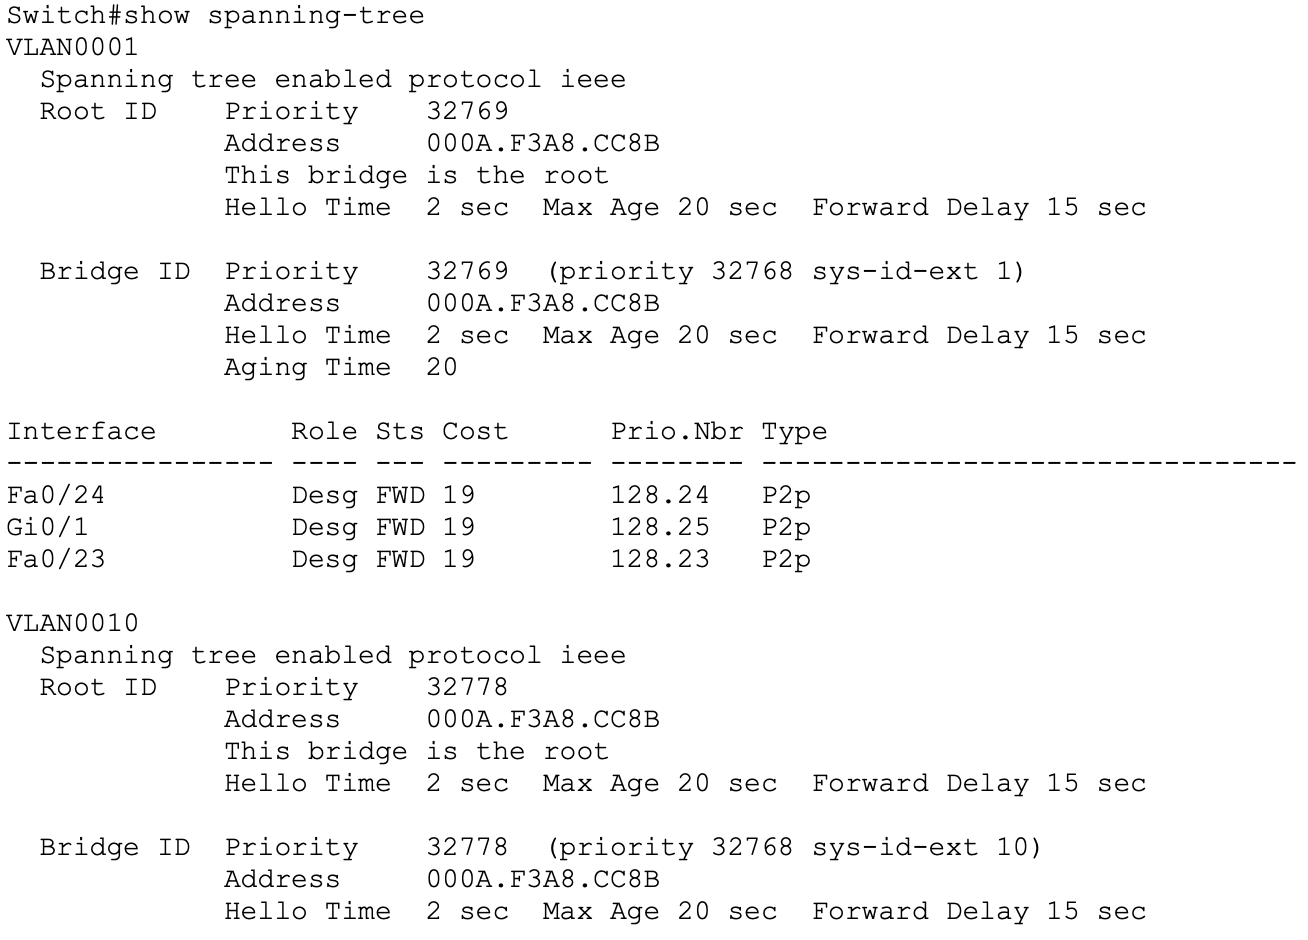
\includegraphics[width=0.85\textwidth]{images/stp/switch-1.png}
  \caption{Информация о STP на первом коммутаторе}
  \label{fig:stp-switch-1}
\end{figure}

\begin{figure}[H]
  \centering
  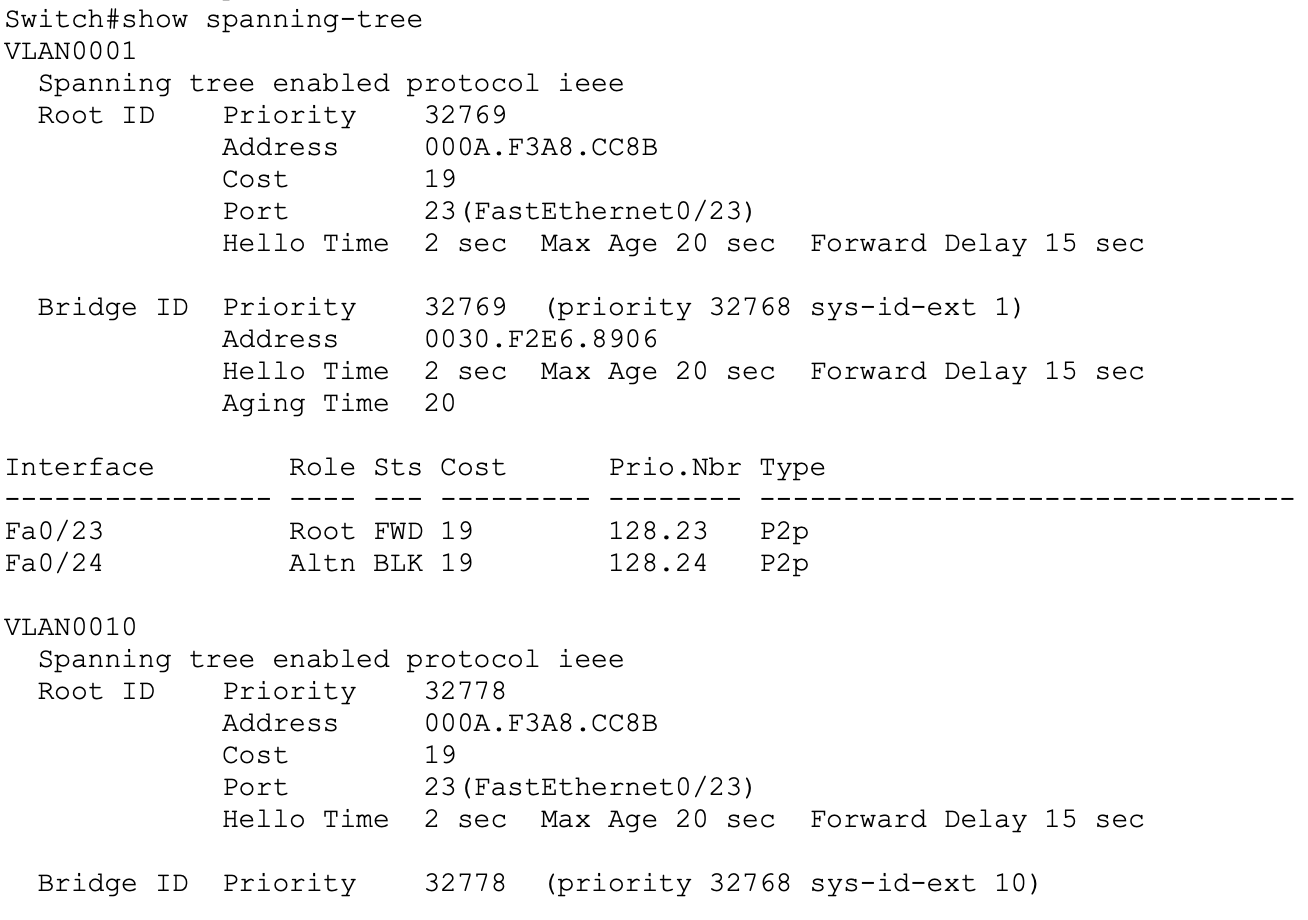
\includegraphics[width=0.85\textwidth]{images/stp/switch-2.png}
  \caption{Информация о STP на втором коммутаторе}
  \label{fig:stp-switch-2}
\end{figure}

\begin{figure}[H]
  \centering
  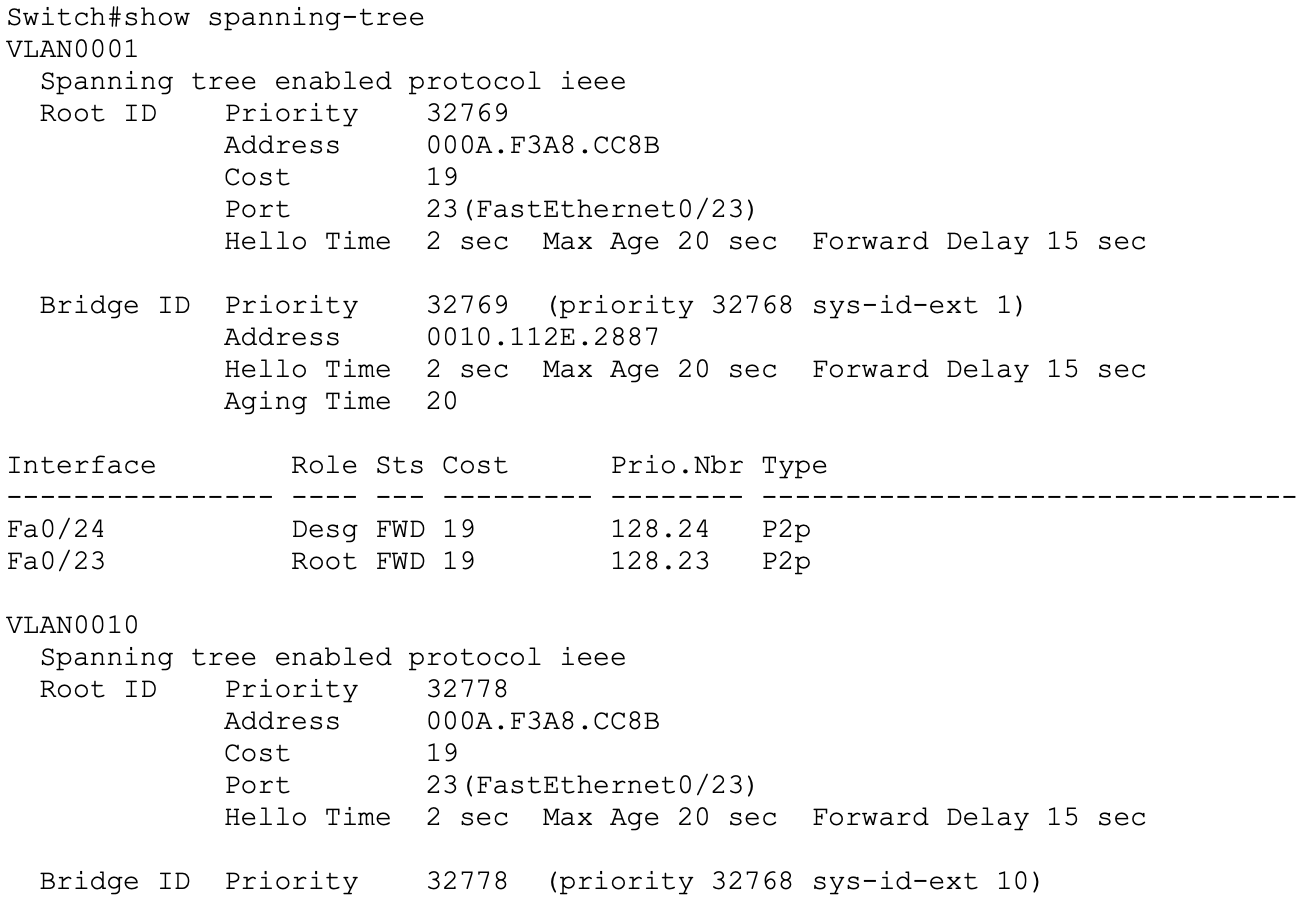
\includegraphics[width=0.85\textwidth]{images/stp/switch-3.png}
  \caption{Информация о STP на третьем коммутаторе}
  \label{fig:stp-switch-3}
\end{figure}

Определим, почему именно первый коммутатор был выбран в качестве корневого.
Рассмотрим приоритеты и MAC-адреса каждого коммутатора (таблица
\ref{tab:stp-switch}).

\begin{table}[H]
  \centering
  \renewcommand*{\arraystretch}{1.25}
  \setlength{\tabcolsep}{12pt}

  \caption{Таблица приоритетов и адресов коммутаторов}
  \label{tab:stp-switch}
  \begin{tabular}{|c|c|c|}
    \hline
    \textbf{№} & \textbf{Приоритет} & \textbf{MAC-адрес}      \\
    \hline
    1          & \texttt{32769}     & \texttt{000A.F3A8.CC8B} \\
    \hline
    2          & \texttt{32769}     & \texttt{0030.F2E6.8906} \\
    \hline
    3          & \texttt{32769}     & \texttt{0010.112E.2887} \\
    \hline
  \end{tabular}
\end{table}

Значение приоритета \texttt{32769} выбрано для каждого из коммутаторов
неслучайно. По умолчанию приоритет вычисляется по формуле: \texttt{32768 + VLAN
  ID}. В этом случае рассматривается VLAN ID равный 1.

Для определения корневого коммутатора используется приоритет и MAC-адрес
устройства. Корневым коммутатором выбирается коммутатор с самым низким
приоритетом, если приоритеты равны, то сравниваются MAC-адреса (тот который
меньше, тот побеждает).

После того, как был определен корневой коммутатор, каждый остальной коммутатор
должен найти один корневой порт, который будет вести к корневому коммутатору.
Чтобы понять, какой порт лучше использовать, каждый некорневой коммутатор
определяет стоимость маршрута от каждого своего порта до корневого коммутатора.
Эта стоимость определяется суммой стоимостей всех устройств, которые нужно
пройти кадру, чтобы дойти до корневого коммутатора. В свою очередь, стоимость
канала определяется по его скорости (чем выше скорость, тем меньше
стоимость). Процесс определения происходит следующим образом:

\begin{enumerate}
  \item корневой коммутатор посылает BPDU с полем Root Path Cost, равным нулю;
  \item ближайший коммутатор определяет скорость порта, на который пришел BPDU,
  и добавляет стоимость согласно таблице \ref{tab:stp-cost};
  \item далее этот второй коммутатор посылает BPDU нижестоящим коммутаторам, но
  уже с новым значением Root Path Cost.
\end{enumerate}

\begin{table}[H]
  \centering
  \renewcommand*{\arraystretch}{1.25}
  \setlength{\tabcolsep}{24pt}

  \caption{Таблица скорости порта и стоимости STP}
  \label{tab:stp-cost}
  \begin{tabular}{|c|c|}
    \hline
    \textbf{Скорость порта} & \textbf{Стоимость STP} \\
    \hline
    10 Mbps                 & 100                    \\
    \hline
    100 Mbps                & 19                     \\
    \hline
    1 Gbps                  & 4                      \\
    \hline
    10 Gbps                 & 2                      \\
    \hline
  \end{tabular}
\end{table}

На рис. \ref{fig:stp-disabled-ports} видно, что на втором коммутаторе был
отключен и назначен резервным порт \texttt{FastEthernet0/24}.

\begin{figure}[H]
  \centering
  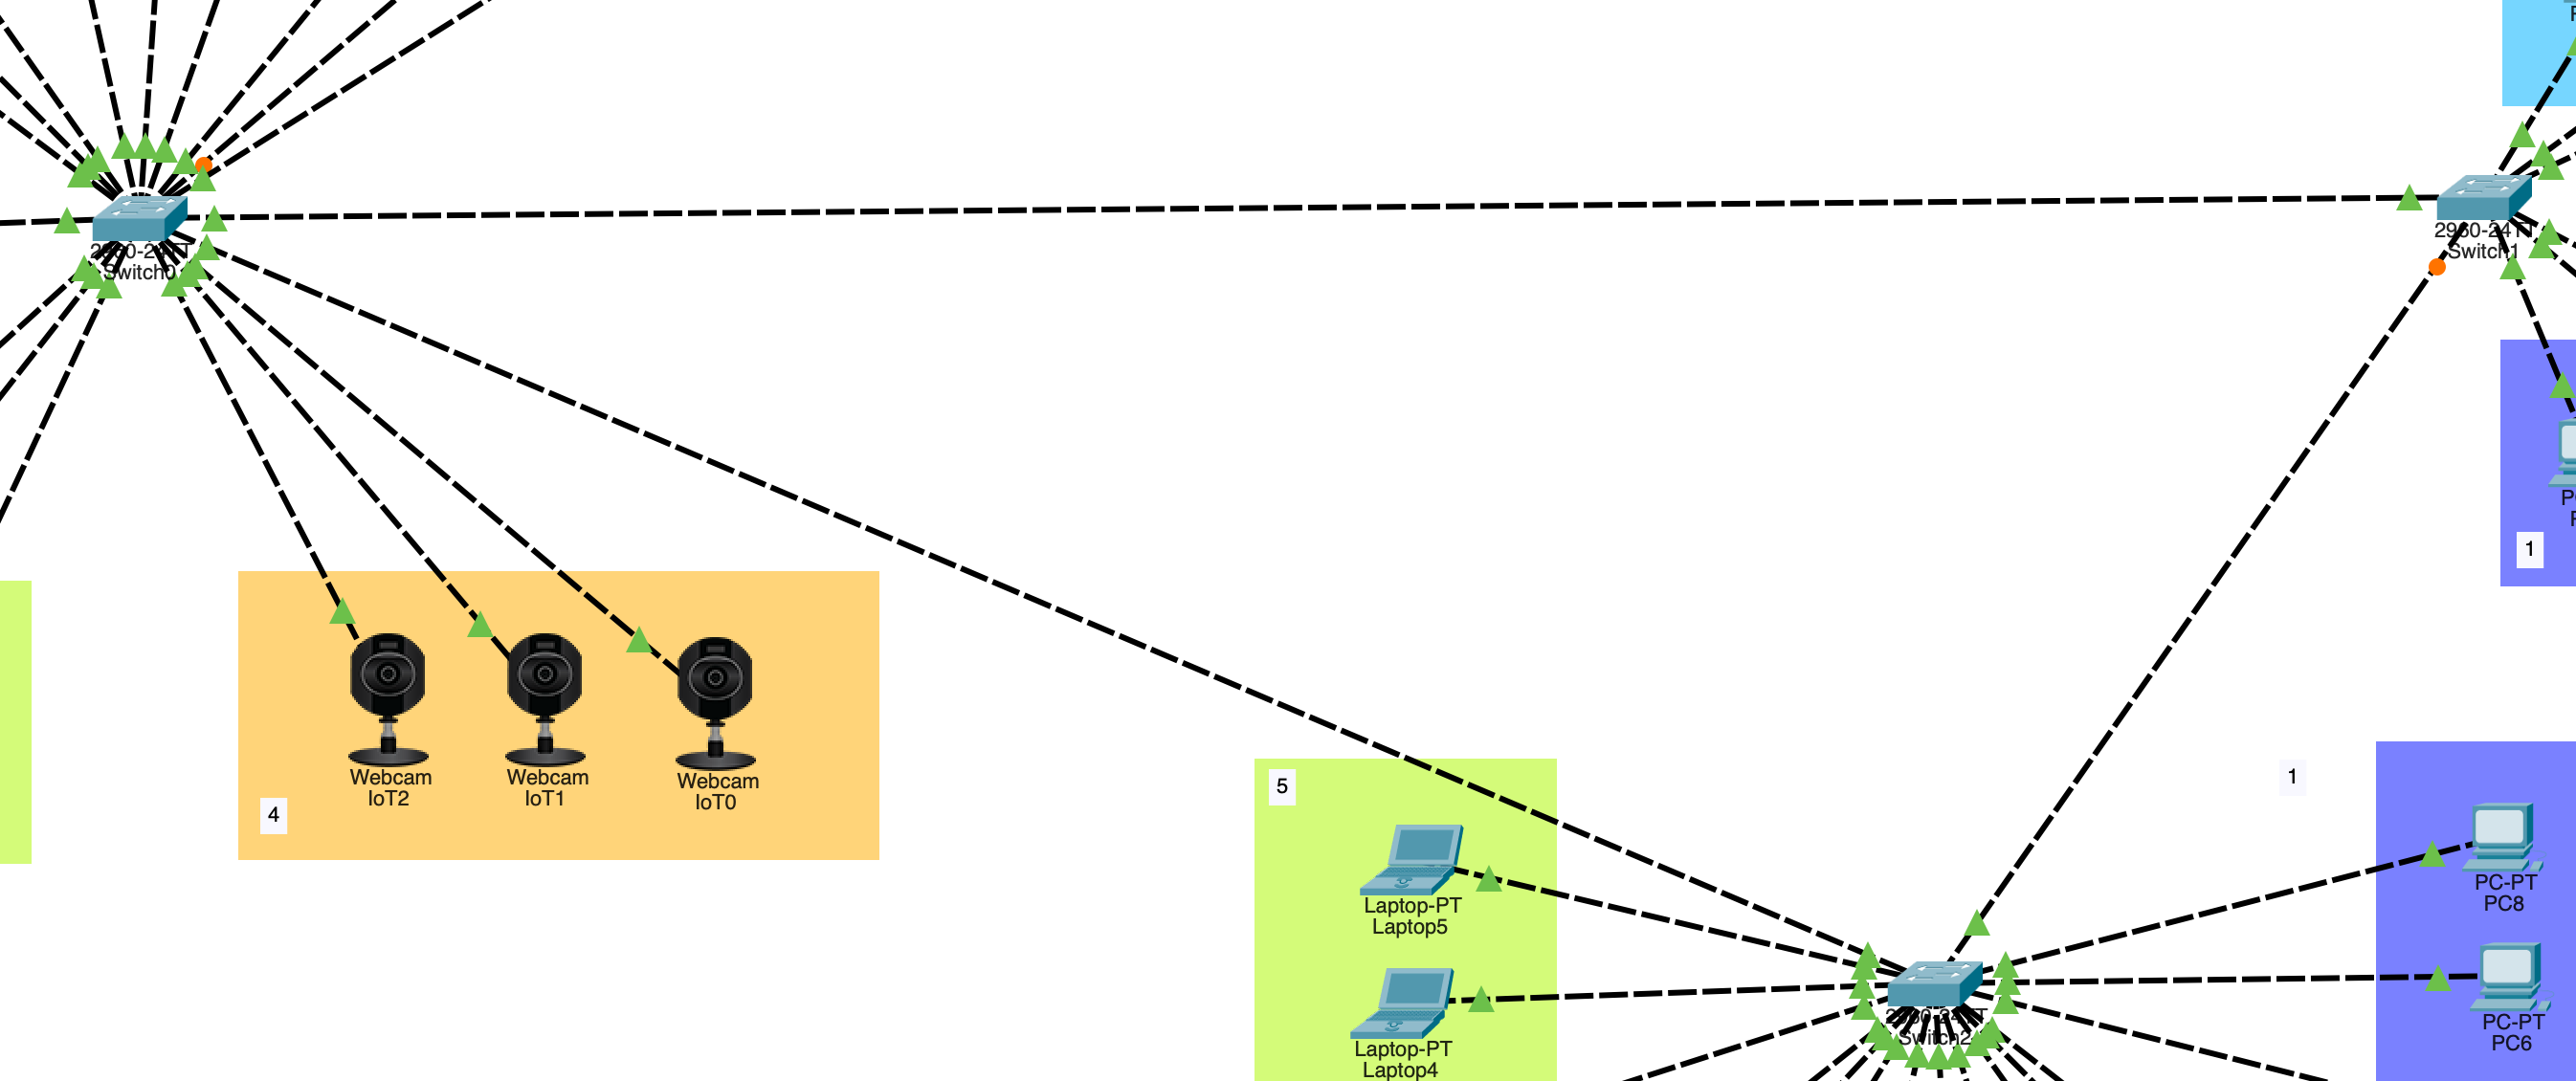
\includegraphics[width=\textwidth]{images/stp/disabled-ports.png}
  \caption{Отключенные порты на коммутаторах}
  \label{fig:stp-disabled-ports}
\end{figure}

В случае, если вручную отключить порт \texttt{FastEthernet0/23} на втором
коммутаторе, то будет использован резервный порт \texttt{FastEthernet0/24} (рис.
\ref{fig:stp-manually-disable-port}).

\begin{figure}[H]
  \centering
  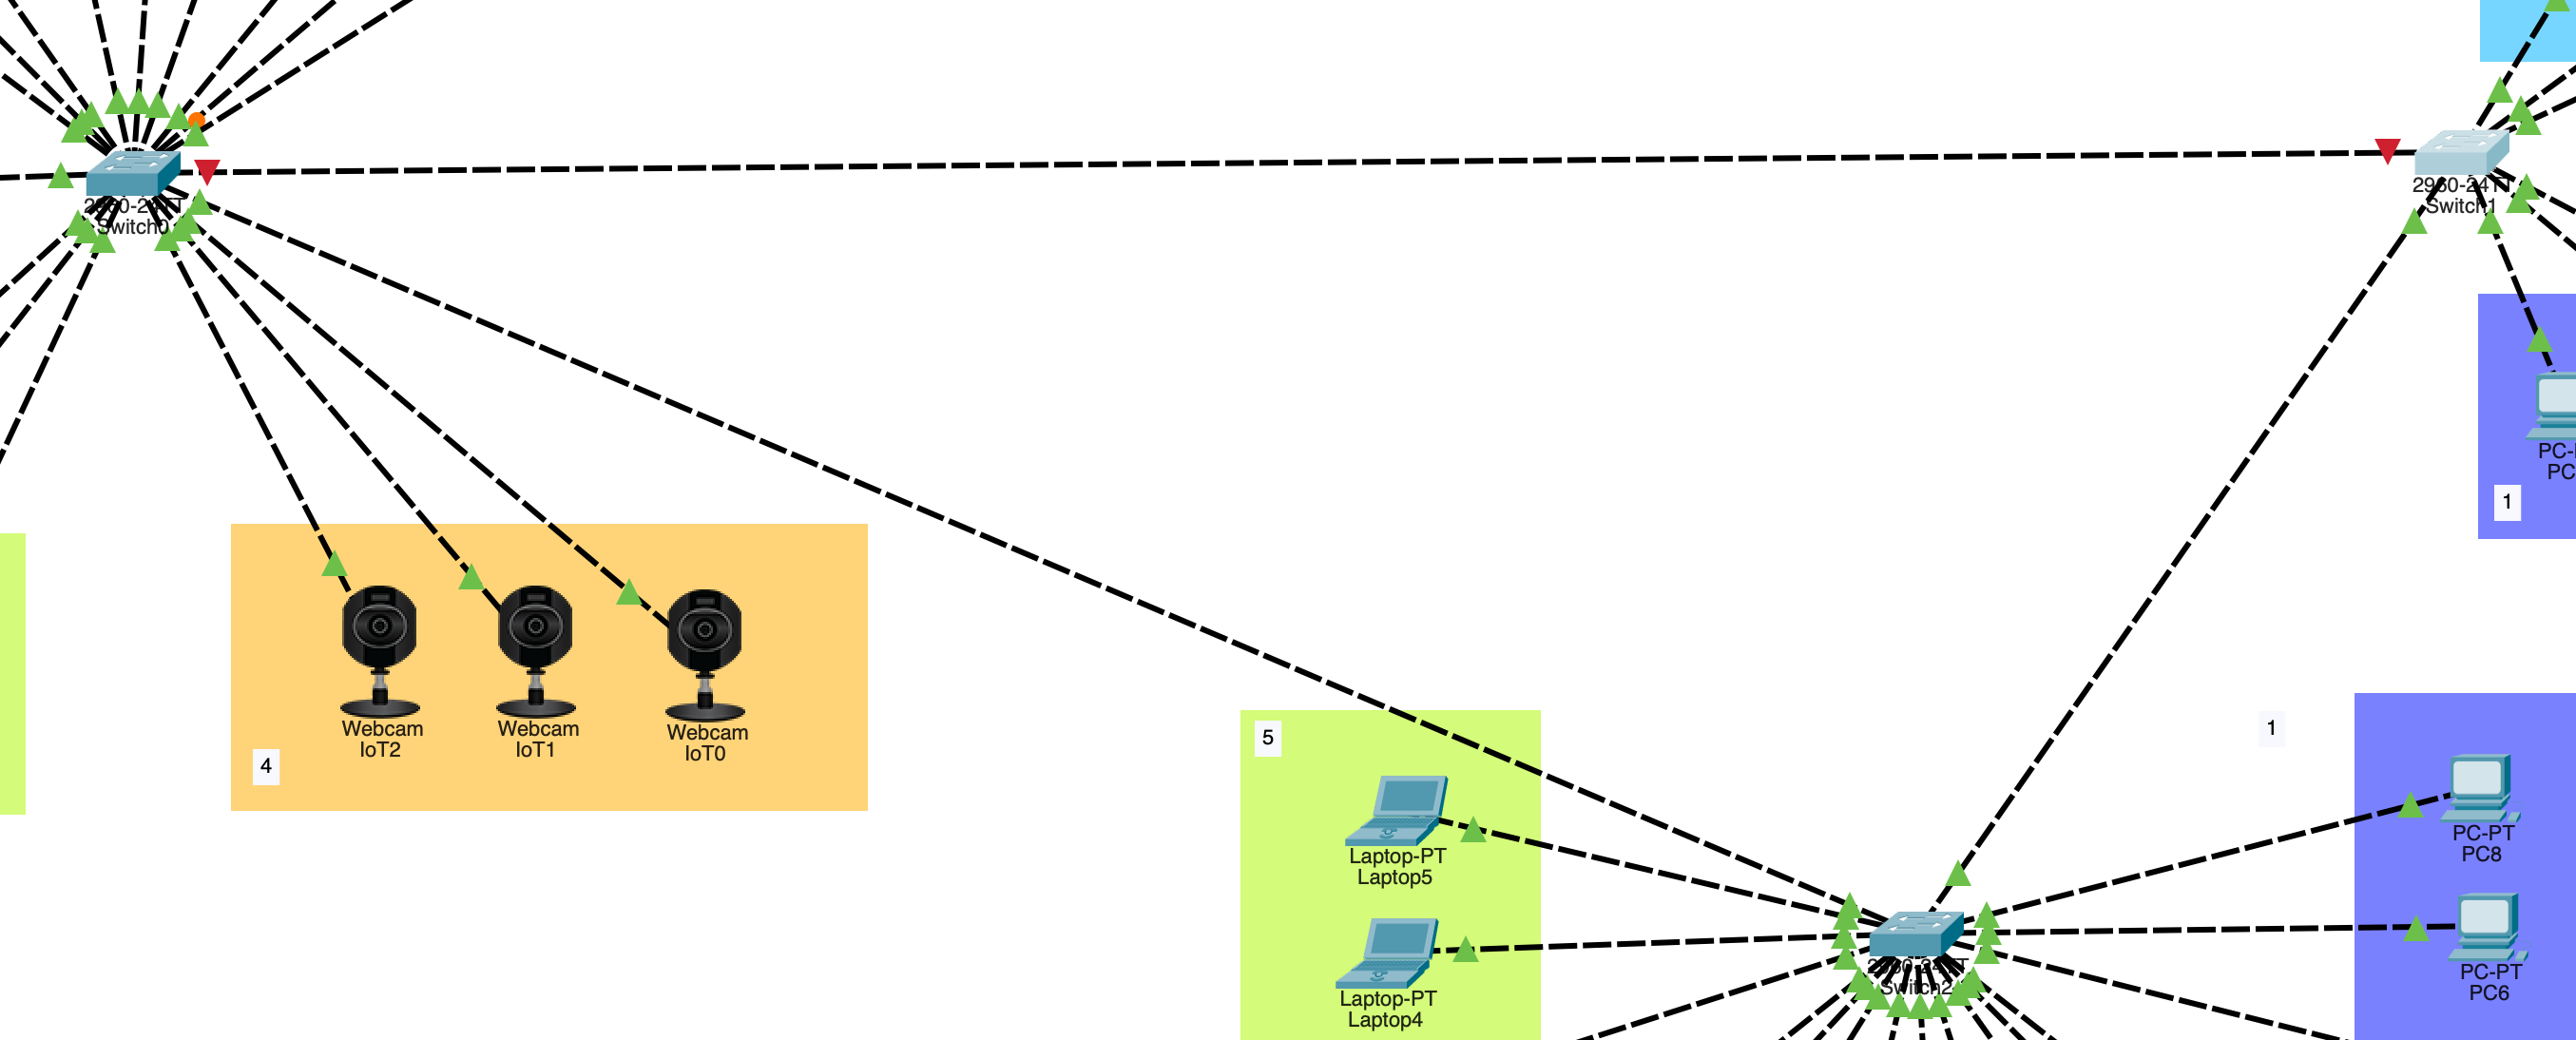
\includegraphics[width=\textwidth]{images/stp/manually-disable-port.png}
  \caption{Использование резервного порта}
  \label{fig:stp-manually-disable-port}
\end{figure}

\subsubsection{Тестирование протокола RSTP}

Поскольку мой вариант соответствует 19 номеру, а остаток от деления на 4 равен
3, то в данном задании мне необходимо создать коммутационную петлю между
коммутатором третьего уровня и соседним с ним коммутатором. В моем случае это
первый коммутатор (рис. \ref{fig:rstp-loop}).

\begin{figure}[H]
  \centering
  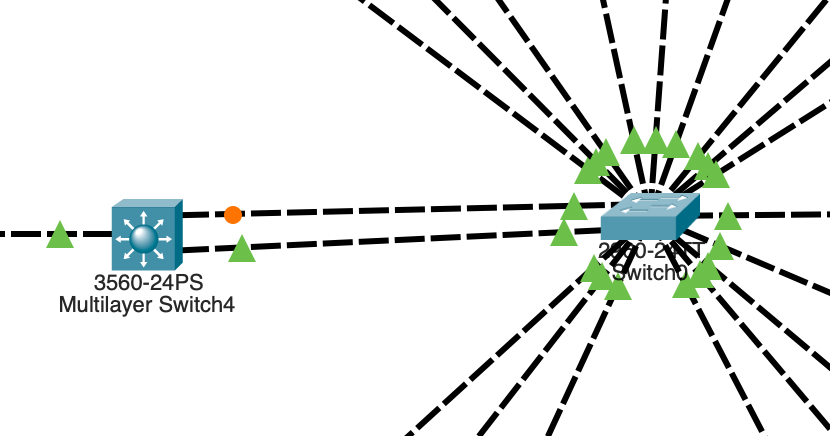
\includegraphics[width=0.7\textwidth]{images/rstp/loop.png}
  \caption{Коммутационная петля между первым коммутатором и коммутатором
    третьего уровня}
  \label{fig:rstp-loop}
\end{figure}

Как видно на рис. \ref{fig:rstp-root}, в качестве корневого коммутатора был
выбран первый коммутатор.

\begin{figure}[H]
  \centering
  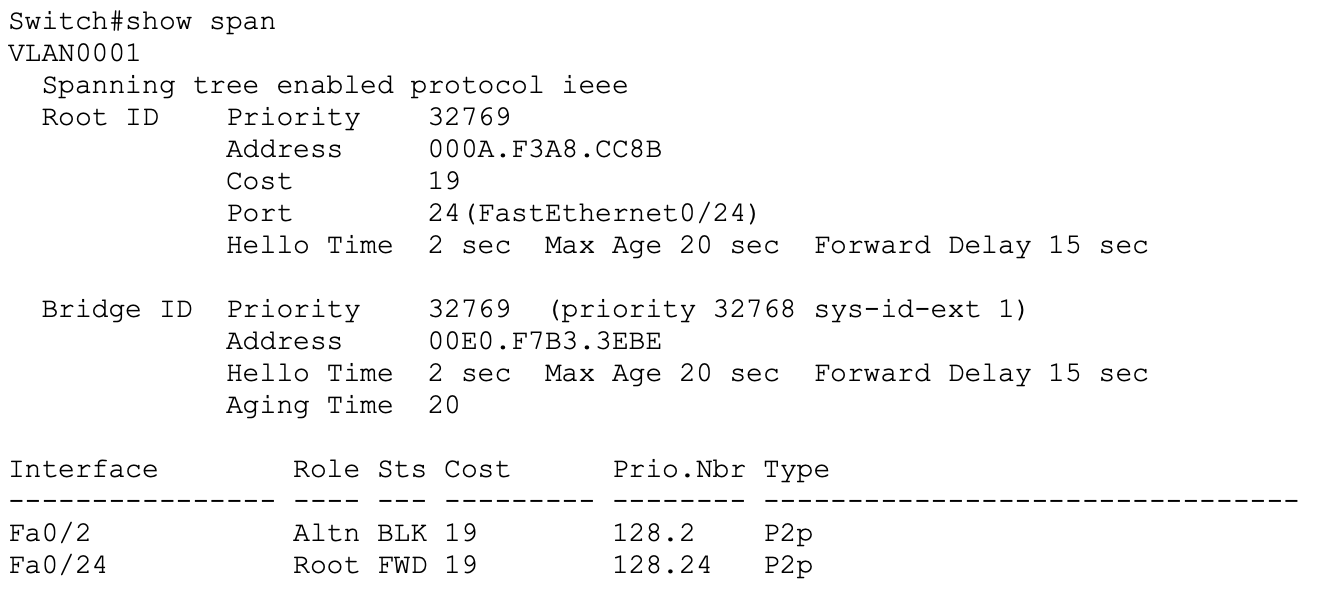
\includegraphics[width=0.9\textwidth]{images/rstp/root.png}
  \caption{Информация о STP на коммутаторе третьего уровня}
  \label{fig:rstp-root}
\end{figure}

Для того, чтобы определить время сходимости при использовании STP, отключим порт
\texttt{FastEthernet0/24} на коммутаторе третьего уровня. Примерно через 30
секунд коммутаторы смогли определить корневой коммутатор между собой.

С помощью команды \texttt{spanning-tree mode rapid-pvst} на обоих коммутаторах
было включено использование RSTP. Теперь при отключении одного из портов
коммутаторы практически моментально сходятся.

\subsection{Работа с протоколом EtherChannel}

\subsubsection{Статическое агрегирование}

В данном задании, поскольку номер моего варианта равен 19, мне необходимо
соединить первый и третий коммутаторы с помощью четырех каналов. Как видно на
рис. \ref{fig:ec-scheme-before}, после подключения коммутатор из-за STP
отключает все порты, кроме одного, чтобы не было коммутационной петли.

С помощью команды \texttt{channel-group 1 mode on} на всех нужных
интерфейсах на каждом из коммутаторов был включен режим агрегирования портов.
Как показано на рис. \ref{fig:ec-scheme-after}, после выполнения данной команды
начали использоваться все порты вместо одного.

\begin{figure}[H]
  \centering
  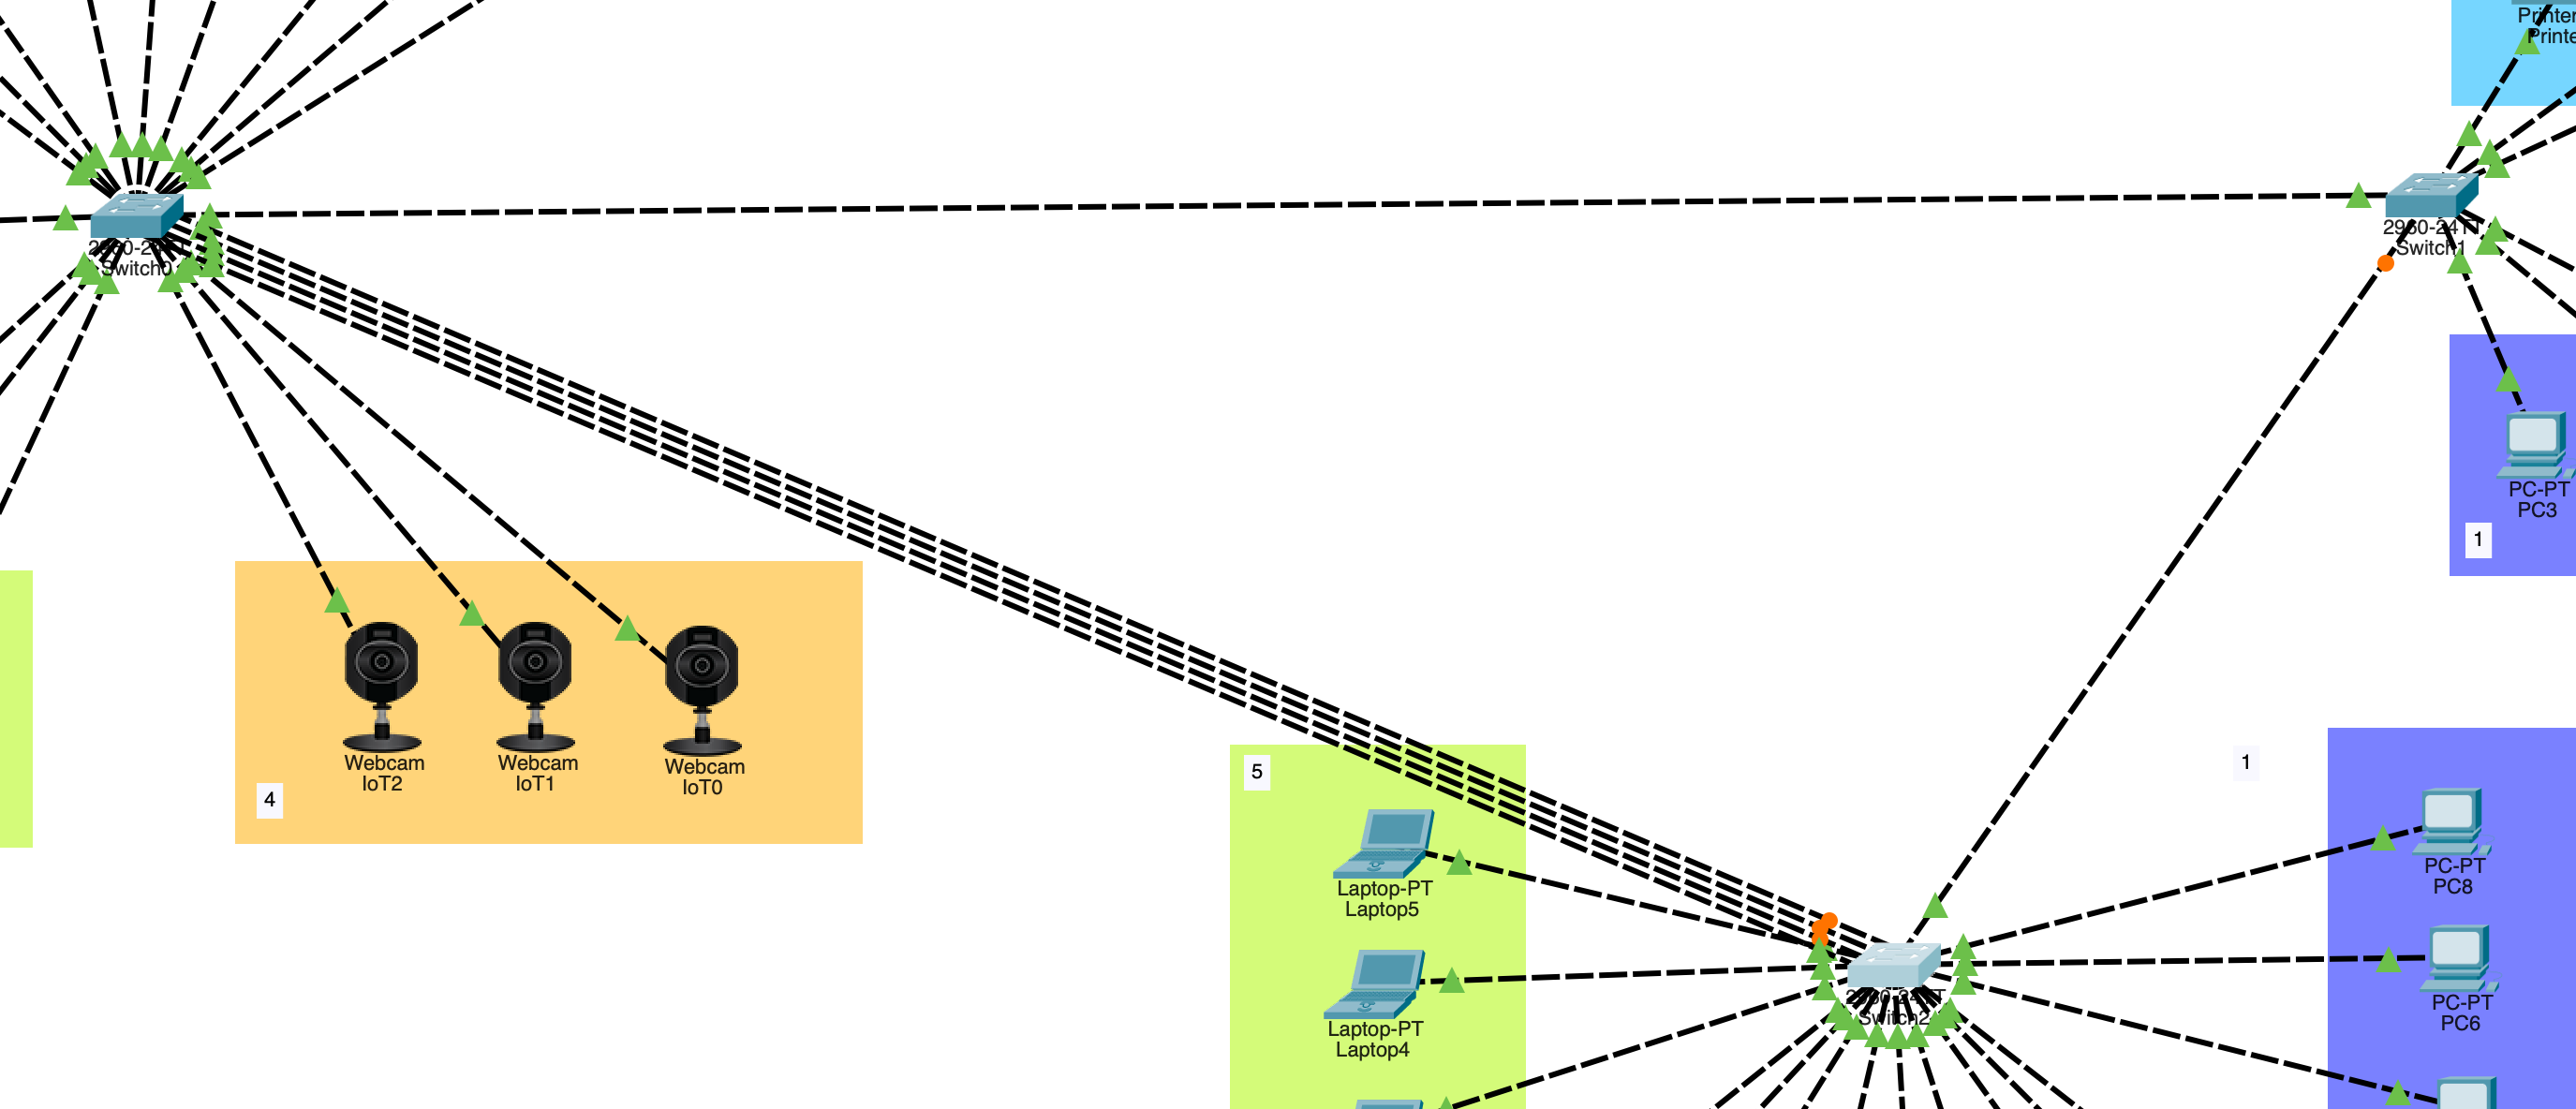
\includegraphics[width=\textwidth]{images/ec/scheme-before.png}
  \caption{Схема соединения коммутаторов}
  \label{fig:ec-scheme-before}
\end{figure}

\begin{figure}[H]
  \centering
  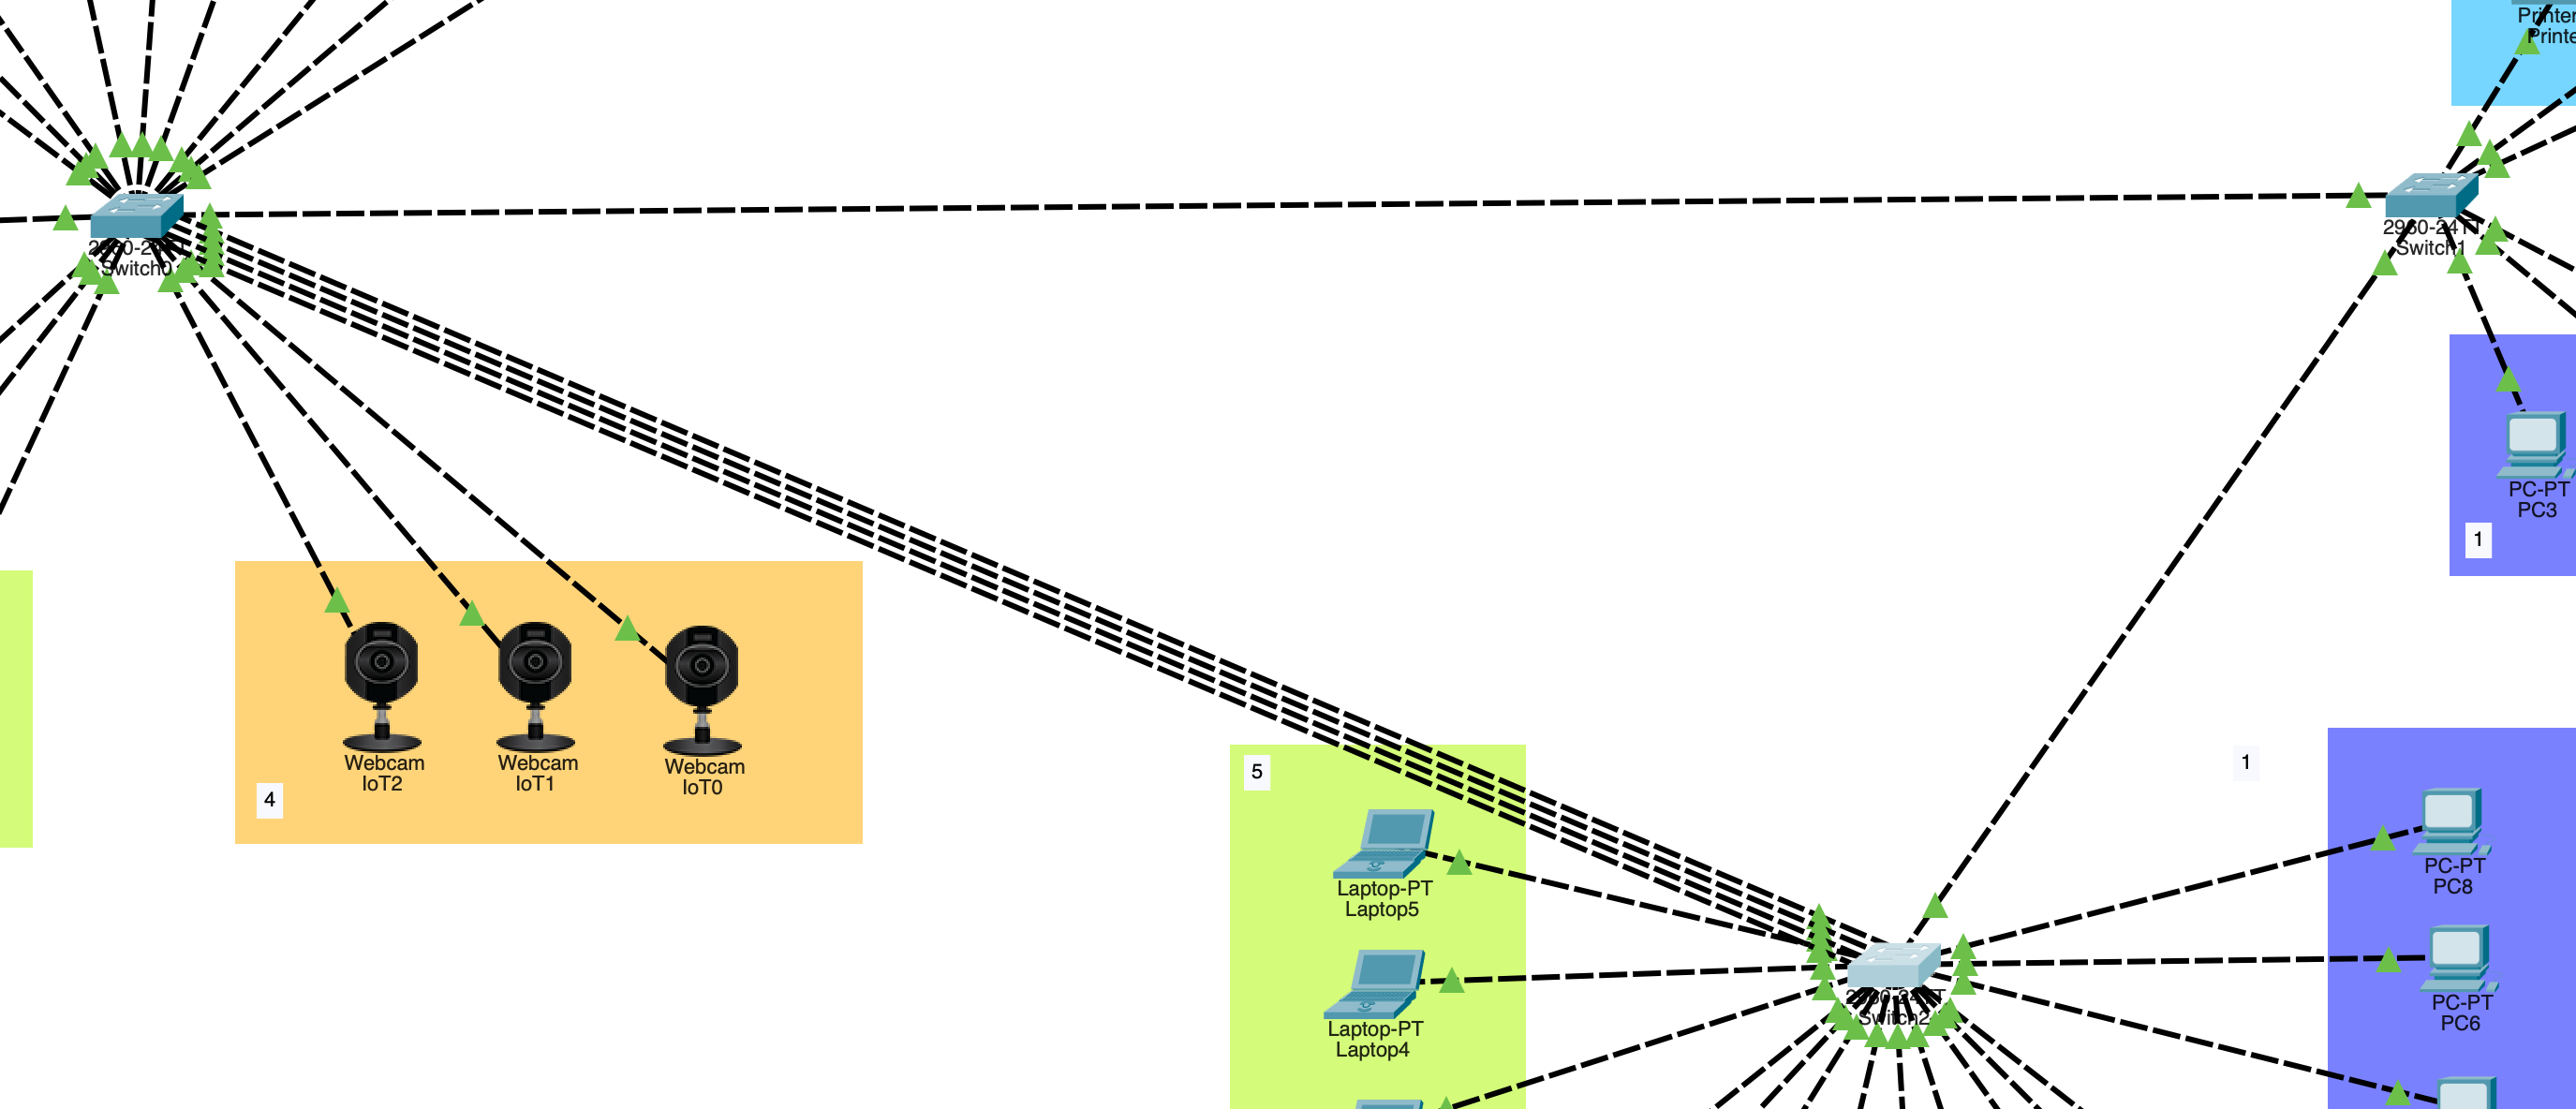
\includegraphics[width=\textwidth]{images/ec/scheme-after.png}
  \caption{Схема соединения коммутаторов}
  \label{fig:ec-scheme-after}
\end{figure}

Чтобы удостовериться в том, что все агрегация портов успешно настроена, была
выполнена команда \texttt{show etherchannel port-channel}. На рис.
\ref{fig:ec-port-channel} видно, что все четыре порта, которые используются для
подключения к другому коммутатору, агрегированы в один канал.

\begin{figure}[H]
  \centering
  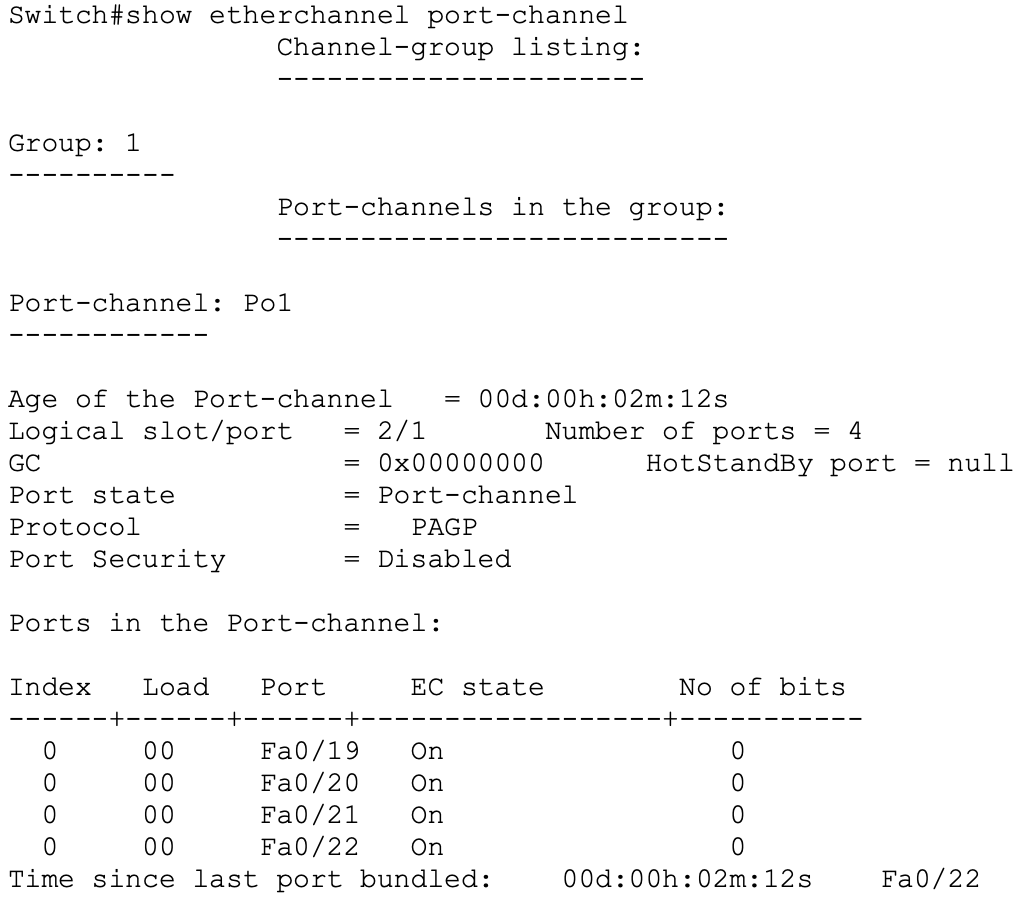
\includegraphics[width=0.8\textwidth]{images/ec/port-channel.png}
  \caption{Информация о агрегации портов}
  \label{fig:ec-port-channel}
\end{figure}

\subsubsection{Динамическое агрегирование LACP}

После соединения всех коммутаторов так, как это указано в задании, получилась
схема, изображенная на рис. \ref{fig:lacp-scheme}. На первом, втором и третьем
коммутаторах на необходимых портах была настроена агрегация каналов с помощью
команды \texttt{channel-group N mode active}, где \texttt{N} --- номер группы
канала. Номера были назначены в соответствии с номером коммутатора, т. е. у
первого коммутатора первый канал, у второго --- второй, у третьего --- третий.
Также данная команда была использована и на соответствующих портах коммутатора
третьего уровня.

\begin{figure}[H]
  \centering
  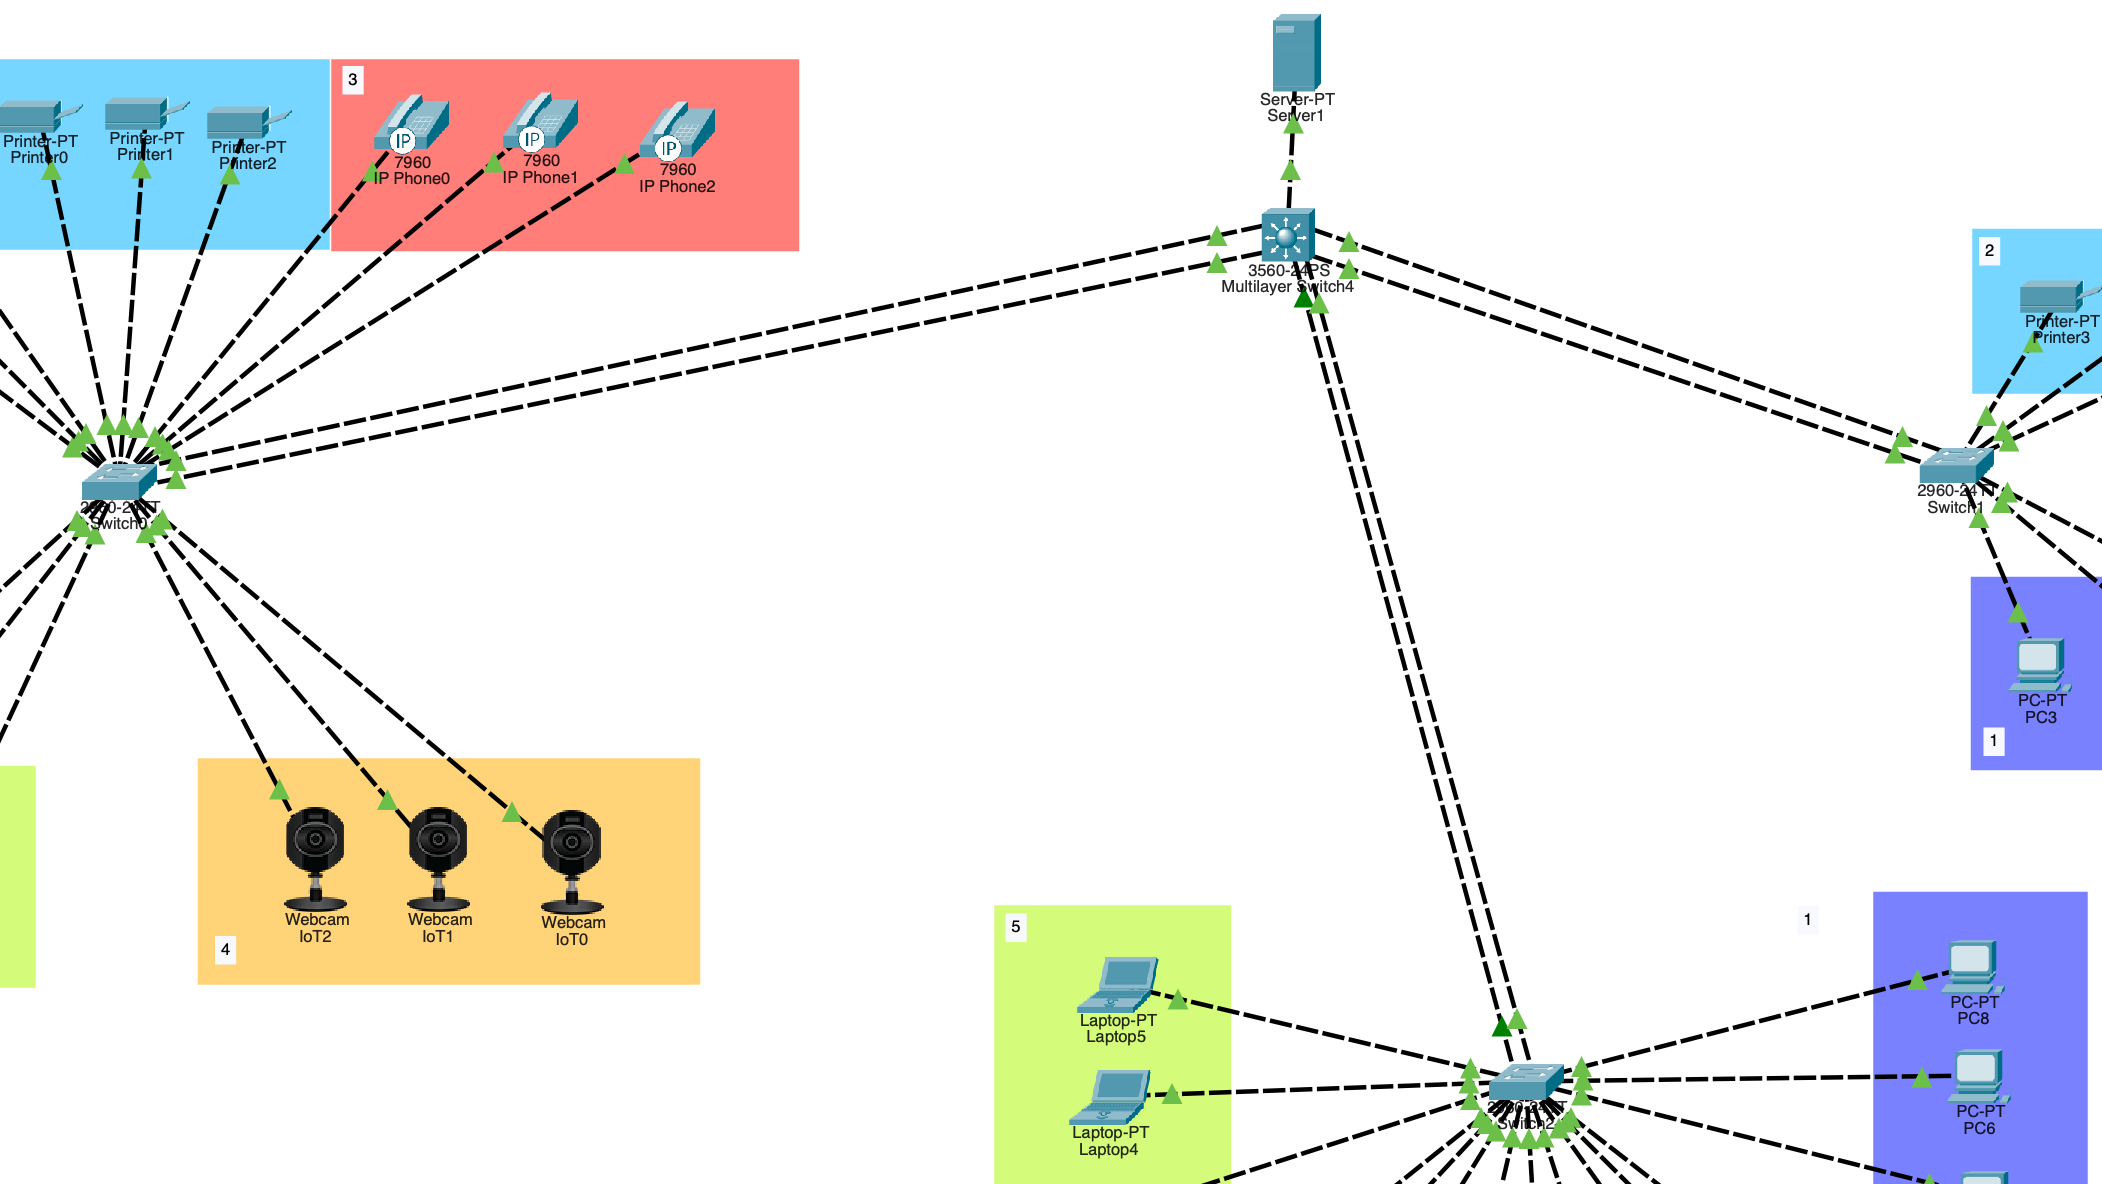
\includegraphics[width=\textwidth]{images/lacp/scheme.png}
  \caption{Схема соединения коммутаторов}
  \label{fig:lacp-scheme}
\end{figure}

С помощью команды \texttt{show etherchannel port-channel} на коммутаторе
третьего уровня была выведена информация о агрегированных портах (рис.
\ref{fig:lacp-channel-1}-\ref{fig:lacp-channel-3}). Как можно видеть, все
порты были успешно агрегированы.

\begin{figure}[H]
  \centering
  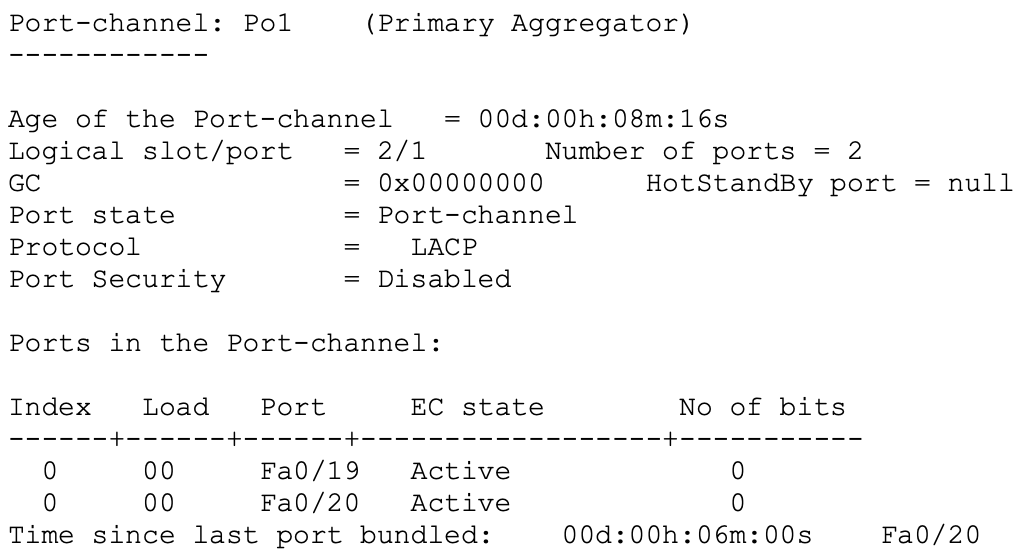
\includegraphics[width=0.8\textwidth]{images/lacp/channel-1.png}
  \caption{Первый канал агрегирования портов}
  \label{fig:lacp-channel-1}
\end{figure}

\begin{figure}[H]
  \centering
  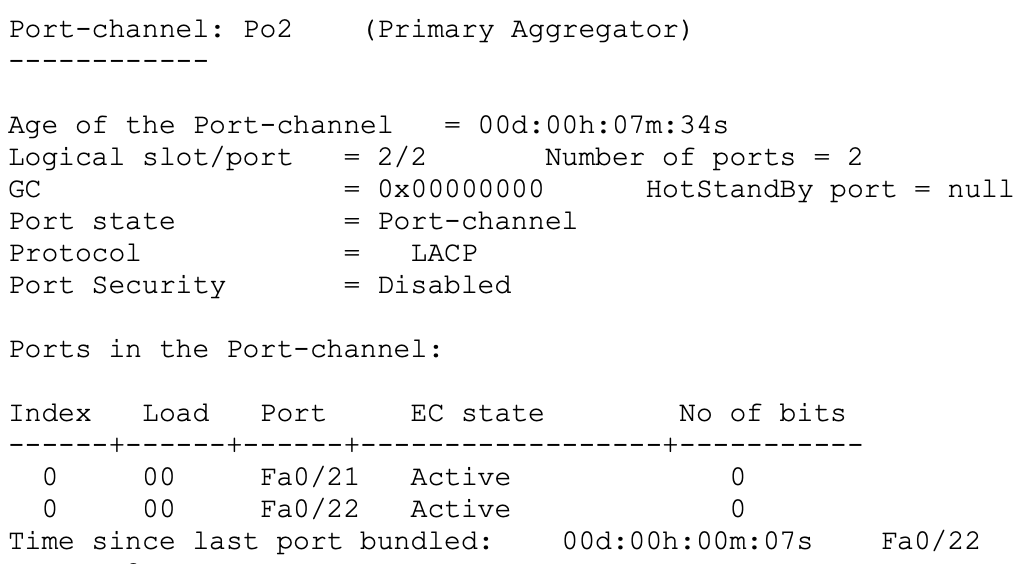
\includegraphics[width=0.8\textwidth]{images/lacp/channel-2.png}
  \caption{Второй канал агрегирования портов}
  \label{fig:lacp-channel-2}
\end{figure}

\begin{figure}[H]
  \centering
  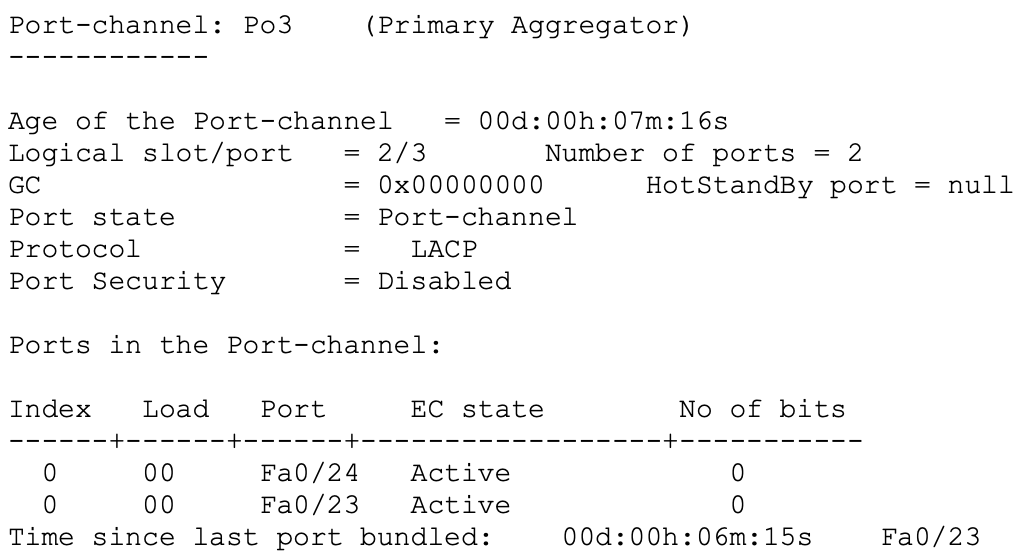
\includegraphics[width=0.8\textwidth]{images/lacp/channel-3.png}
  \caption{Третий канал агрегирования портов}
  \label{fig:lacp-channel-3}
\end{figure}

\section{Заключение}

В ходе выполнения данной лабораторной работы я изучил и практически ознакомился
с основными принципами работы концентраторов и коммутаторов второго уровня в
компьютерных сетях, а также организовал отказоустойчивой сети на основе
коммутаторов.

\end{document}
